% ===========================================================================
%  Panel Review 1 -- 23CSE498 Project Phase 2 -- Team 50
%  Zero Trust-Enabled SDN for Secure Load Balancing in Edge Networks
%
%  Compile from inside ppt/ (twice, for the TOC/agenda):
%      cd ppt && pdflatex -interaction=nonstopmode sections_1_2_3.tex
%
%  FIGURES
%    figures/uml_*.png     PlantUML, sources in ppt/uml/, built by ./build_uml.sh
%    ../base_model/...     real plotted data, regenerated 2026-09-08
%    ../data/figures/...   RAFT failover, regenerated 2026-09-08
%  Nothing here is a copied snapshot: every plot is referenced at its source so
%  it cannot drift from the recording it was made from. The old fig8/fig9 are
%  deliberately NOT used -- their numbers were hard-coded literals from a run
%  that has since been superseded.
%
%  NUMBERS: every figure on every slide comes from the 2026-09-08 re-score
%  (data/comparison/comparison.txt, data/nfr_report.txt, and the evaluation
%  reports). Do not hand-edit a number here without regenerating its source.
%
%  STILL TO FILL IN: the four MOOC course titles, and logo.png.
% ===========================================================================
\documentclass[aspectratio=169, 11pt]{beamer}

% --- Packages & Setup ---
\usepackage[utf8]{inputenc}
\usepackage[T1]{fontenc}
\usepackage{xcolor}
\usepackage{booktabs}
\usepackage{array}
\usepackage{graphicx}
\usepackage{tikz} % Required for the corner box
\usetikzlibrary{calc}

\graphicspath{{./}{../}{figures/}}

% Try loading Open Sans; fallback if missing
\IfFileExists{opensans.sty}{\usepackage[default,scale=0.95]{opensans}}{}

% --- Branding Colors ---
\definecolor{amritaMaroon}{HTML}{A4123F}

% --- Theme Setup ---
\usetheme{Madrid}
\usecolortheme[named=amritaMaroon]{structure}
\setbeamertemplate{navigation symbols}{}
\setbeamertemplate{footline}[frame number]
% Madrid's headline is a full section bar; on a 28-frame deck it eats the
% vertical space the figures need, so it is dropped.
\setbeamertemplate{headline}{}
\setbeamerfont{frametitle}{size=\normalsize}
\setbeamerfont{framesubtitle}{size=\tiny}
\setbeamercolor{block title}{bg=amritaMaroon!12,fg=amritaMaroon}
\setbeamercolor{block body}{bg=amritaMaroon!5}
\setbeamertemplate{itemize items}[circle]

% \FIXME marks the placeholders that must be filled in before the review.
\newcommand{\FIXME}[1]{\textcolor{red}{\textbf{#1}}}
% \rubric is the discreet marks tag carried by the slides that earn them.
\newcommand{\rubric}[1]{Rubric: #1}
% \src cites the artifact a number came from.
\newcommand{\src}[1]{{\color{gray}\tiny [#1]}}

% \fitfig scales a figure to the frame body; height binds for the wide plots.
\providecommand{\fitfig}[2][0.74]{%
  \centerline{\includegraphics[width=\textwidth,height=#1\textheight,keepaspectratio]{#2}}}

\begin{document}

% ============================================================ TITLE SLIDE
\begin{frame}
    \begin{tikzpicture}[remember picture,overlay]
        \node[fill=amritaMaroon, text=white, font=\bfseries\footnotesize, anchor=north east, rounded corners=2pt, inner sep=5pt]
        at ($(current page.north east) + (-0.2cm,-0.2cm)$)
        {Type 3: Software Project};
    \end{tikzpicture}

    \centering
    % logo.png is the 1948x568 Amrita wordmark; the guard keeps the build alive
    % if it is ever moved. logo_square.png is only 97 px, so it is not used.
    \IfFileExists{logo.png}{
\includegraphics[width=5.4cm]{logo.png}}{%
      \fbox{\begin{minipage}{5.4cm}\centering\vspace{3pt}\scriptsize \FIXME{logo.png}\vspace{3pt}\end{minipage}}}
    \vspace{0.10cm}

    {\large \textbf{\textcolor{amritaMaroon}{Zero Trust-Enabled SDN for Secure Load Balancing in Edge Networks}}} \\
    \vspace{0.05cm}
    {\footnotesize \textbf{23CSE498 -- Project Phase 2 (Panel Review 1)} \quad | \quad \textbf{Team Number: 50}} \\
    \vspace{0.12cm}

    \begin{table}
        \centering
        \scriptsize
        \renewcommand{\arraystretch}{1.05}
        \begin{tabular}{|c|c|l|}
            \hline
            \textbf{S.No} & \textbf{Register Number} & \textbf{Student Name} \\
            \hline
            1 & CB.SC.U4CSE23262 & K R Jeevan Raj \\
            \hline
            2 & CB.SC.U4CSE23303 & Aravind Kumar M \\
            \hline
            3 & CB.SC.U4CSE23307 & Arjun Krishnakumar \\
            \hline
            4 & CB.SC.U4CSE23308 & Ashwin Kumar RM \\
            \hline
            5 & CB.SC.U4CSE23544 & Bhuvanesh S \\
            \hline
        \end{tabular}
    \end{table}
    \vspace{0.08cm}

    {\footnotesize Guide: \textbf{Dr. Radhika N}, Professor, Department of CSE} \\
    \vspace{0.06cm}
    {\scriptsize \today}
\end{frame}

% ============================================================ AGENDA
\section{Agenda}
\begin{frame}{Agenda}
    \vspace{2pt}
    \begin{columns}[T]
      \begin{column}{0.5\textwidth}
        \footnotesize
        \begin{enumerate}\itemsep4pt
          \item \textbf{Introduction} --- the edge setting, and what we built
          \item \textbf{Motivation} --- why self-reported telemetry fails
          \item \textbf{Literature Survey} --- what exists, and the gap
          \item \textbf{Problem Statement \& Objectives}
        \end{enumerate}
      \end{column}
      \begin{column}{0.5\textwidth}
        \footnotesize
        \begin{enumerate}\itemsep4pt
          \setcounter{enumi}{4}
          \item \textbf{Architecture} of the proposed framework
          \item \textbf{Solution} --- the two rails and their enforcement
          \item \textbf{Results} --- a controlled two-arm comparison
          \item \textbf{Limitations} and technical enrichment
        \end{enumerate}
      \end{column}
    \end{columns}

    \vspace{10pt}
    \begin{block}{\footnotesize The one sentence}
      \footnotesize
      Every load balancer in production decides where to send work from what the
      servers \emph{say about themselves}; we built an SDN control plane that
      decides from what it \emph{observes}, revokes a misbehaving server in the
      data plane in under a second, and measured the difference against a
      complete no-zero-trust control arm.
    \end{block}
\end{frame}

% ============================================================ INTRODUCTION
\section{Introduction}

\begin{frame}{1. Introduction: The Edge Setting}
    \begin{columns}[T]
      \begin{column}{0.56\textwidth}
        \scriptsize
        Edge computing pushes computation onto gateways, roadside units,
        factory-floor servers and campus racks. \textbf{Three facts collide there:}
        \begin{enumerate}\itemsep3pt
          \item \textbf{The perimeter model fails.} A node \emph{inside} the
                network can be compromised, rented, misconfigured or simply selfish.
          \item \textbf{Self-reported telemetry is the norm, and is gameable.}
                Kubernetes, cloud auto-scalers and MEC orchestrators all schedule
                on what a node says about itself. A node that under-reports load
                \emph{attracts} traffic.
          \item \textbf{Zero Trust is a doctrine, not a mechanism.} NIST SP
                800-207 mandates continuous verification but specifies no way for
                a control plane to verify the \emph{serving infrastructure} and
                act on the result in the data path.
        \end{enumerate}
        \vspace{4pt}
        \textbf{Scope we are careful about:} this is \emph{demonstrated in an
        emulated network}, never ``proven in production''.
      \end{column}
      \begin{column}{0.44\textwidth}
        \centering
        \vspace{6pt}
        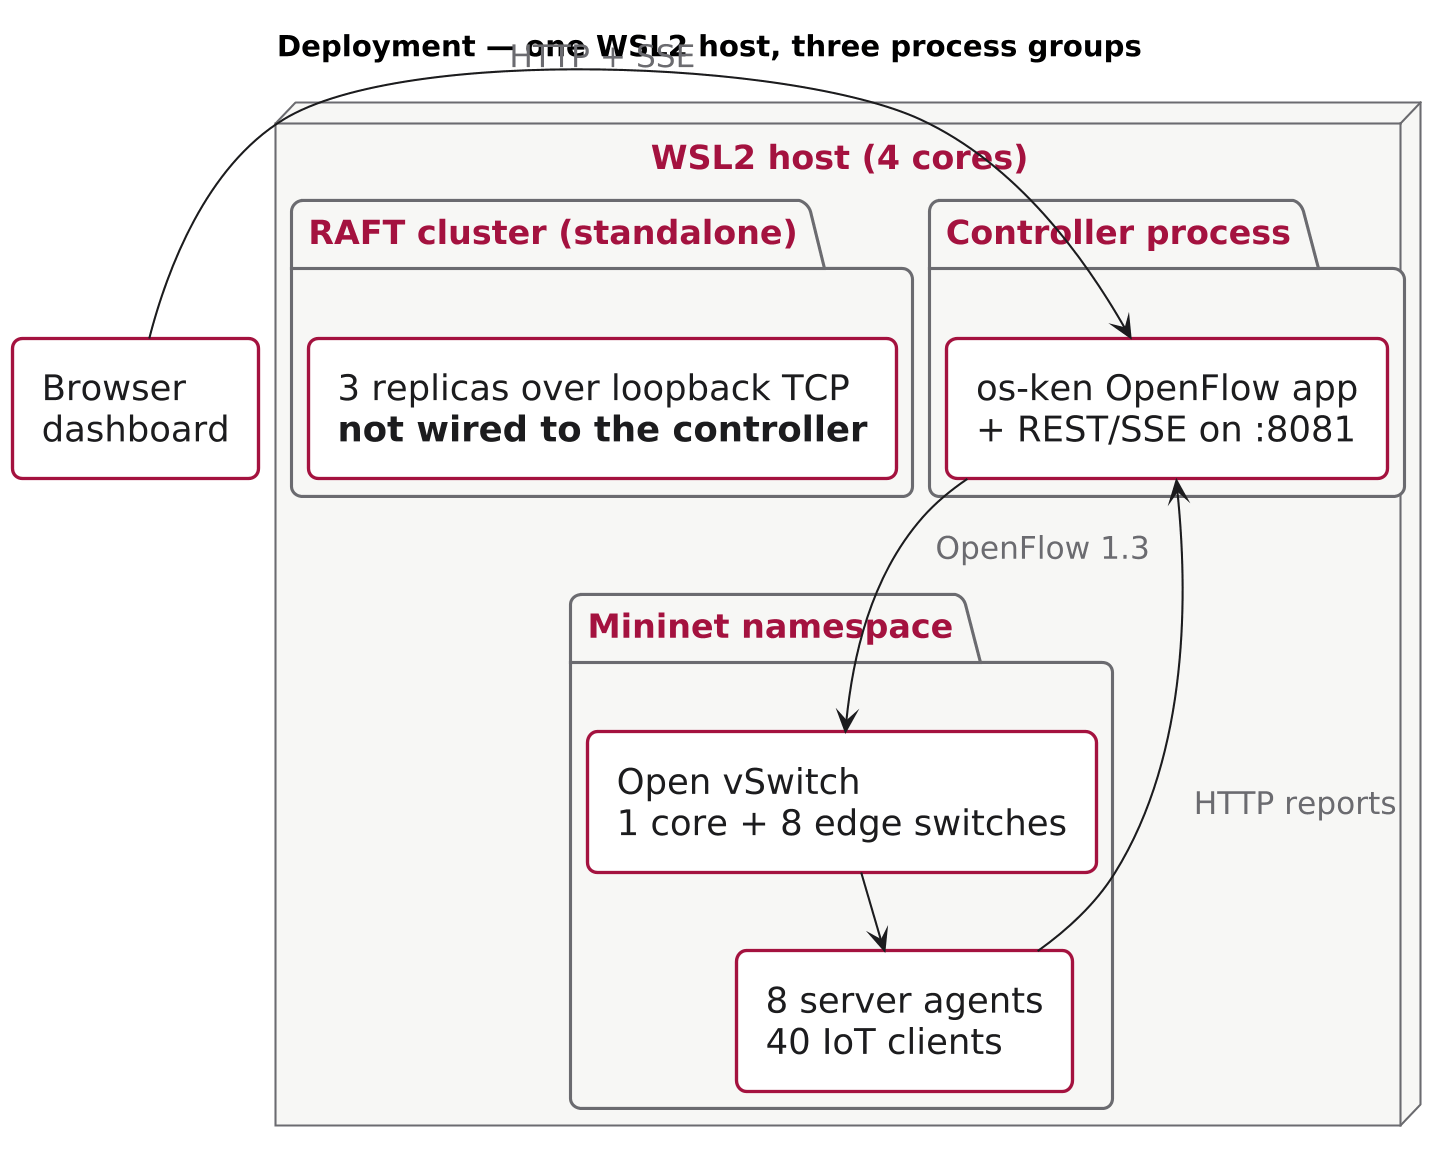
\includegraphics[width=\textwidth,height=0.62\textheight,keepaspectratio]{figures/uml_deployment.png}
      \end{column}
    \end{columns}
\end{frame}

\begin{frame}{1. Introduction: What We Built}
    \framesubtitle{\rubric{UML Diagrams, DB Schema, APIs, Module Interaction \& Deployment (5 Marks)}}
    \scriptsize
    An SDN control plane that scores every edge server on \textbf{measured
    behaviour}, and when a server misbehaves \textbf{revokes it in the data plane}
    as real OpenFlow rules, while an append-only cryptographic ledger records why.

    \vspace{6pt}
    \begin{columns}[T]
      \begin{column}{0.5\textwidth}
        \textbf{The system under test}
        \begin{itemize}\itemsep2pt
          \item os-ken OpenFlow 1.3 controller application
          \item Northbound REST + SSE API on \texttt{:8081}
          \item Live dashboard, tamper-testable ledger ribbon
        \end{itemize}
        \vspace{4pt}
        \textbf{The test harness} (not the product)
        \begin{itemize}\itemsep2pt
          \item Mininet + Open vSwitch topology
          \item Server agents doing \emph{real bounded work}
          \item IoT clients and the attack simulator
        \end{itemize}
      \end{column}
      \begin{column}{0.5\textwidth}
        \textbf{Scale of one run}
        \begin{itemize}\itemsep2pt
          \item 1 core + 8 edge OVS switches
          \item 8 edge servers, 40 IoT devices
          \item 6 armed attack classes, delayed onset
          \item $\approx$300\,s per run, 4-core WSL2 box
          \item $\approx$27\,000 recorded events per run
        \end{itemize}
        \vspace{4pt}
        \textbf{Why it is an experiment:} we built a complete
        \emph{no-zero-trust} version of the same system, launched by the same
        code. Most projects compare against a \emph{description} of a baseline
        rather than a running one.
      \end{column}
    \end{columns}
\end{frame}

% ============================================================ MOTIVATION
\section{Motivation}

\begin{frame}{2. Motivation: The Attacker Does Not Need Cryptography}
    \scriptsize
    \begin{block}{\footnotesize The core observation}
      \footnotesize
      Almost every real orchestrator schedules on what nodes \emph{claim} about
      themselves. A node that under-reports its load therefore \textbf{attracts}
      traffic --- which is exactly what an attacker wants.
      \textbf{The attacker does not have to break any cryptography to do this.
      It just has to lie in a field that everybody believes.}
    \end{block}

    \vspace{4pt}
    \begin{columns}[T]
      \begin{column}{0.5\textwidth}
        \textbf{Why the doctrine does not close it}\\[3pt]
        NIST SP 800-207 says \emph{never trust, always verify, continuously}.
        But commercial Zero-Trust products overwhelmingly verify \textbf{users
        and client devices at access time}. Verifying the \textbf{serving
        infrastructure itself, continuously, with consequences in the routing
        path}, is much less settled. That is the gap this project works in.
      \end{column}
      \begin{column}{0.5\textwidth}
        \textbf{Where it bites in the real world}\\[3pt]
        \emph{MEC / multi-tenant edge:} an operator can host a tenant's workload
        on a node it does not fully control and still bound its exposure ---
        traffic is revoked in under a second, with a signed record of why.\\[3pt]
        \emph{Operational technology:} the scenario that keeps OT engineers awake
        is not a machine that stops --- alarms fire for that --- it is a
        controller that keeps ``working'' while lying about its state, because
        every safety decision downstream is computed from that state.
      \end{column}
    \end{columns}
\end{frame}

\begin{frame}{2. Motivation: Threat Model}
    \framesubtitle{Controller trusted; edge servers and IoT clients untrusted; adversaries non-adaptive}
    \centering\scriptsize
    \begin{tabular}{@{}llll@{}}
      \toprule
      \textbf{Adversary} & \textbf{Subject} & \textbf{Behaviour} & \textbf{Detection signal}\\
      \midrule
      Sybil / load-lying & edge server & under-reports load to attract work & CPU-honesty deviation\\
      Blackhole          & edge server & accepts then drops every task      & timeout rate\\
      Grayhole           & edge server & drops a fraction (0.5) of tasks    & elevated timeout rate\\
      On-off             & edge server & alternates good and bad, 20\,s period & intermittent latency + timeouts\\
      DDoS flood         & IoT client  & floods requests at $\approx$24$\times$ normal rate & per-client request rate\\
      Identity spoof     & IoT client  & claims another device's identity   & source-IP pin mismatch\\
      Bad credentials    & IoT client  & wrong PRESENT-80 key               & challenge-response failure\\
      \bottomrule
    \end{tabular}

    \vspace{7pt}
    \begin{columns}[T]
      \begin{column}{0.5\textwidth}
        \textbf{In scope.} All seven above, armed on a delayed onset so the
        system must detect a \emph{change}, not a static configuration.
      \end{column}
      \begin{column}{0.5\textwidth}
        \textbf{Out of scope, stated before being asked.} Collusion,
        slow-and-low, adaptive attackers that learn our thresholds, and attacks
        on the controller itself.
      \end{column}
    \end{columns}
\end{frame}

% ============================================================ LITERATURE SURVEY
\section{Literature Survey}

\begin{frame}{3. Literature Survey: Five Threads}
    \centering\tiny
    \begin{tabular}{@{}p{0.19\textwidth}p{0.20\textwidth}p{0.55\textwidth}@{}}
      \toprule
      \textbf{Thread} & \textbf{Key sources} & \textbf{What we took from it}\\
      \midrule
      Zero Trust \& trust-aware edge
        & [1] NIST SP 800-207, [11] Ali 2023, [12] TREN 2025, [13] Huang 2024, [19] ETSI MEC
        & [1] is the doctrine we implement \emph{and} the gap we claim. [11] is the closest prior work --- same three ingredients --- but stops at the access decision. [13] is the score-only design whose arithmetic ceiling our Finding 1 characterises.\\
      \addlinespace[2pt]
      Load balancing
        & [2] Mitzenmacher 2001, [14] Azar 1999, [3] Mitzenmacher 2000, [4] Dahlin 2000, [9] Jain 1984, [20] Little 1961
        & [2] is the source of our argmax $\to$ power-of-two-choices fix. [4] \textbf{explains the one place we lose}: stale least-loaded is worse than random. [9] is the fairness index we report.\\
      \addlinespace[2pt]
      Crypto, ledger \& consensus
        & [5] PRESENT 2007, [18] ISO/IEC 29192-2, [6] Merkle 1988, [7] RAFT 2014
        & [5] is the admission cipher, checked against published test vectors. [7] gives the safety properties our RAFT tests are written against --- crash-fault tolerant, \emph{not} Byzantine.\\
      \addlinespace[2pt]
      SDN platform
        & [8] OpenFlow 2008, [10] Mininet 2010
        & [8] is the source of Finding 3: once a rule is installed, matching packets never return to the controller. [10] is why we say ``emulated'', never ``production''.\\
      \addlinespace[2pt]
      Learning \& method
        & [15] UCB1 2002, [16] Wilcoxon 1945, [17] Holm 1979, [21] Nygard 2018
        & [15] is the online weight optimiser --- a classical bandit, \emph{not} deep RL. [16],[17] are the paired test and the multiple-comparison correction. [21]'s circuit breaker is our probation mechanism.\\
      \bottomrule
    \end{tabular}
\end{frame}

\begin{frame}{3. Literature Survey: Positioning, and the Gap}
    \centering\scriptsize
    \begin{tabular}{@{}p{0.22\textwidth}p{0.40\textwidth}p{0.28\textwidth}@{}}
      \toprule
      \textbf{System} & \textbf{Reported headline} & \textbf{Enforcement}\\
      \midrule
      Ali, Gregory \& Li (2023) [11] & F1 94.3\,\% anomaly detection; 96.1\,\% access-decision accuracy & access decision\\
      TREN (2025) [12]               & 95\,\% detection accuracy; $-$20\,\% latency; $+$25\,\% throughput & policy enforcement\\
      Huang et al.\ (2024) [13]      & $+$13.37 to 21.87\,\% malicious-node detection rate & trust-based selection\\
      \textbf{This work}             & \textbf{97.9\,\% over 48 subjects} (8 classes); 8/8 detected; 0/40 honest mislabelled & \textbf{OpenFlow drop rules}\\
      \bottomrule
    \end{tabular}

    \vspace{5pt}
    \begin{block}{\scriptsize Read this as positioning, not as a benchmark}
      \scriptsize
      Cross-paper numbers in this area are \textbf{not comparable} and we do not
      present them as though they were. An ``accuracy'' over a two-class
      DDoS/Sybil problem and one over an eight-class problem with 40 honest
      subjects are not the same quantity.
    \end{block}

    \vspace{3pt}
    \scriptsize
    \textbf{The gap.} The systems above report how well a trust mechanism
    \emph{performs}. \textbf{None reports a limit of the trust mechanism itself.}
    A system reporting 95\,\% detection from a single trust rail cannot tell
    whether its remaining 5\,\% is noise or a structural blind spot ---
    which is exactly what our Finding 1 identifies.
\end{frame}

% ============================================================ PROBLEM & OBJECTIVES
\section{Problem Statement \& Objectives}

\begin{frame}{4. Problem Statement}
    \vspace{4pt}
    \begin{block}{\footnotesize Research question}
      \normalsize
      \centering
      \textbf{Can an SDN control plane continuously verify edge servers using
      \emph{observed} rather than \emph{claimed} behaviour, and enforce the
      verdict in the data plane fast enough to matter?}
    \end{block}

    \vspace{8pt}
    \scriptsize
    \begin{columns}[T]
      \begin{column}{0.5\textwidth}
        \textbf{What has to be true for the answer to be yes}
        \begin{itemize}\itemsep2pt
          \item Verification must run on evidence the node cannot forge ---
                measured outcomes, not telemetry
          \item The verdict must reach the \emph{data plane}, not just a
                scheduler's preference ordering
          \item It must be fast enough that an attacker's window is bounded
          \item The record must be tamper-evident after the fact
        \end{itemize}
      \end{column}
      \begin{column}{0.5\textwidth}
        \textbf{Our answer, at prototype scale}\\[3pt]
        \textbf{Yes} --- with isolation inside a 3-second bound --- and with the
        important \textbf{negative result} that score-based trust alone is
        provably \emph{insufficient} to do it.\\[5pt]
        That negative result is the part we would most want carried forward,
        and it is developed on the next slides.
      \end{column}
    \end{columns}
\end{frame}

\begin{frame}{4. Objectives}
    \scriptsize
    \begin{enumerate}\itemsep3pt
      \item \textbf{Characterise the insufficiency of score-based trust.} Derive
            the trust floor for a non-degrading liar analytically, verify it
            against the shipped calculator, and demonstrate it in a live run.
      \item \textbf{Show the two rails are complementary, not redundant.} A trust
            score and an independent anomaly gate must each catch attackers the
            other misses.
      \item \textbf{Enforce trust verdicts in the data plane with measured
            bounds} --- OpenFlow drop rules and VIP rewrites, timed end to end.
      \item \textbf{Compare against a running control arm}, not a description of
            one, plus a statistically grounded multi-baseline study with
            correction and effect sizes --- \emph{including the comparisons we lose}.
      \item \textbf{Make the trust record tamper-evident} with forensic
            resolution, so an edit is localised rather than merely detected.
      \item \textbf{Establish whether the routing weights can be learned online},
            and report the result honestly either way.
      \item \textbf{Separate selection strategy from hardware as the scaling
            limit} --- determine what actually stops the fleet scaling.
    \end{enumerate}
\end{frame}

% ============================================================ ARCHITECTURE
\section{Architecture of the Proposed Framework}

\begin{frame}{5. Architecture: Five Layers, One Process}
    \framesubtitle{\rubric{UML Diagrams, DB Schema, APIs, Module Interaction \& Deployment (5 Marks)}}
    \fitfig[0.70]{figures/uml_architecture.png}
    \vspace{1pt}
    \centering\tiny
    The trust engine and the ledger are \textbf{libraries the controller calls
    in-process}, not separate services. That is what lets the control arm remove
    enforcement without becoming a second codebase.
\end{frame}

\begin{frame}{5. Architecture: Module Interaction}
    \framesubtitle{\rubric{UML Diagrams, DB Schema, APIs, Module Interaction \& Deployment (5 Marks)}}
    \fitfig[0.74]{figures/uml_components.png}
\end{frame}

\begin{frame}{5. Architecture: API and Data Model}
    \framesubtitle{\rubric{UML Diagrams, DB Schema, APIs, Module Interaction \& Deployment (5 Marks)}}
    \centering\tiny
    \begin{tabular}{@{}llll@{}}
      \toprule
      \textbf{Method} & \textbf{Path} & \textbf{Request} & \textbf{Response}\\
      \midrule
      POST & \texttt{/auth/challenge}  & \texttt{\{device\_id\}}                  & \texttt{\{nonce\}}, 64-bit, TTL 30\,s\\
      POST & \texttt{/auth/verify}     & \texttt{\{device\_id, response\}}        & \texttt{\{token\}} \;\textbar\; \textbf{403} \texttt{auth\_denied\{kind\}}\\
      POST & \texttt{/report}          & \texttt{\{status, latency\_ms, \ldots\}} & task outcome; \texttt{client\_ip} from the socket\\
      POST & \texttt{/register}        & \texttt{\{node\_id, concurrency\}}       & agent start-up registration\\
      POST & \texttt{/topology/links}  & \texttt{\{links:[\ldots]\}}              & link parameters the harness built\\
      GET  & \texttt{/trust/score}     & \texttt{?node\_id=}                      & \texttt{\{node\_id: score\}} or all nodes\\
      GET  & \texttt{/node/status}     & \texttt{?node\_id=}                      & \texttt{TrustState.snapshot()}\\
      GET  & \texttt{/ledger/verify}   & none                                     & \texttt{\{valid, chain\_length, batch\}}\\
      GET  & \texttt{/api/events}      & none                                     & Server-Sent Events stream\\
      \bottomrule
    \end{tabular}

    \vspace{6pt}
    \begin{columns}[T]
      \begin{column}{0.5\textwidth}
        \scriptsize
        \textbf{No relational database.} The \textbf{ledger} is the store of
        record for trust, and its integrity is \emph{cryptographic} --- SHA-256
        chain plus a Merkle root per block --- rather than referential. The JSONL
        recording is the durable evidence log; configuration is YAML.
      \end{column}
      \begin{column}{0.5\textwidth}
        \scriptsize
        \textbf{Why SSE and not WebSockets.} It is one-way, plain HTTP, and needs
        no third-party library --- which matters because the target machine is
        apt-only Python 3.14 with \textbf{no pip, no venv and no web framework}.
      \end{column}
    \end{columns}
\end{frame}

% ============================================================ SOLUTION
\section{Solution}

\begin{frame}{6. Solution: Zero Trust as Three Gates}
    \framesubtitle{\rubric{Software Architecture, Implementation, Integration \& Tech Stack (5 Marks)}}
    \fitfig[0.66]{figures/uml_zero_trust_gates.png}
    \vspace{2pt}
    \centering\tiny
    Measured at the gates in the live run: identity refused \textbf{3} devices
    (2 wrong-key, 1 spoof); continuous verification raised \textbf{291} anomalies;
    graduated response applied \textbf{39} quarantines and \textbf{21} re-steers.
    \src{data/comparison/comparison.txt}
\end{frame}

\begin{frame}{6. Solution: The Trust Model, and Its Limit}
    \framesubtitle{\rubric{Software Architecture, Implementation, Integration \& Tech Stack (5 Marks)}}
    \begin{columns}[T]
      \begin{column}{0.47\textwidth}
        \scriptsize
        \textbf{The formula}
        \[ T = \alpha \bar{R} + \beta \bar{B} + \gamma \bar{H} - \delta \bar{A} \]
        $\alpha{=}0.35$ reliability, $\beta{=}0.25$ behaviour,
        $\gamma{=}0.25$ honesty, $\delta{=}0.15$ anomaly.
        EMA $\lambda{=}0.85$, initial trust 0.5, isolation threshold \textbf{0.30}.

        \vspace{5pt}
        \textbf{Now consider a competent liar} --- a node that lies about its
        load but still serves every task correctly:
        \[ T = 0.35(1.0) + 0.25(0.96) + 0.25(0) - 0.15(1.0) \]
        \[ \mathbf{T = 0.44} \;>\; 0.30 \]
        $\delta$ can only ever subtract 0.15. \textbf{Dishonesty alone can never
        push the score across the isolation line.}
      \end{column}
      \begin{column}{0.53\textwidth}
        \scriptsize
        \begin{block}{\scriptsize Finding 1 --- a characterised insufficiency}
          \scriptsize
          Score-based trust is \textbf{insufficient} for Zero Trust's
          continuous-verification requirement. An independent anomaly gate
          ($\bar{A} \ge 0.5 \Rightarrow$ quarantine regardless of $T$) is
          \textbf{necessary, not belt-and-braces}.
        \end{block}
        \vspace{3pt}
        \textbf{Confirmed live, not just on paper.} In this run the sybil
        attacker srv3 ended at \textbf{$T = 0.699$} --- more than twice the
        isolation threshold --- and was caught \emph{only} by the anomaly gate.
        The blackhole srv6 was caught \emph{only} by the trust score.
        \textbf{Neither rail alone catches both.} \src{comparison.txt}

        \vspace{4pt}
        \textbf{Why this is a contribution, not a bug report.} We kept the
        published formula byte-for-byte and added a documented gate beside it.
        Quietly retuning the weights until the demo worked would have destroyed
        the finding.
      \end{column}
    \end{columns}
\end{frame}

\begin{frame}{6. Solution: Secure Load Balancing}
    \framesubtitle{\rubric{Software Architecture, Implementation, Integration \& Tech Stack (5 Marks)}}
    \begin{columns}[T]
      \begin{column}{0.40\textwidth}
        \centering
        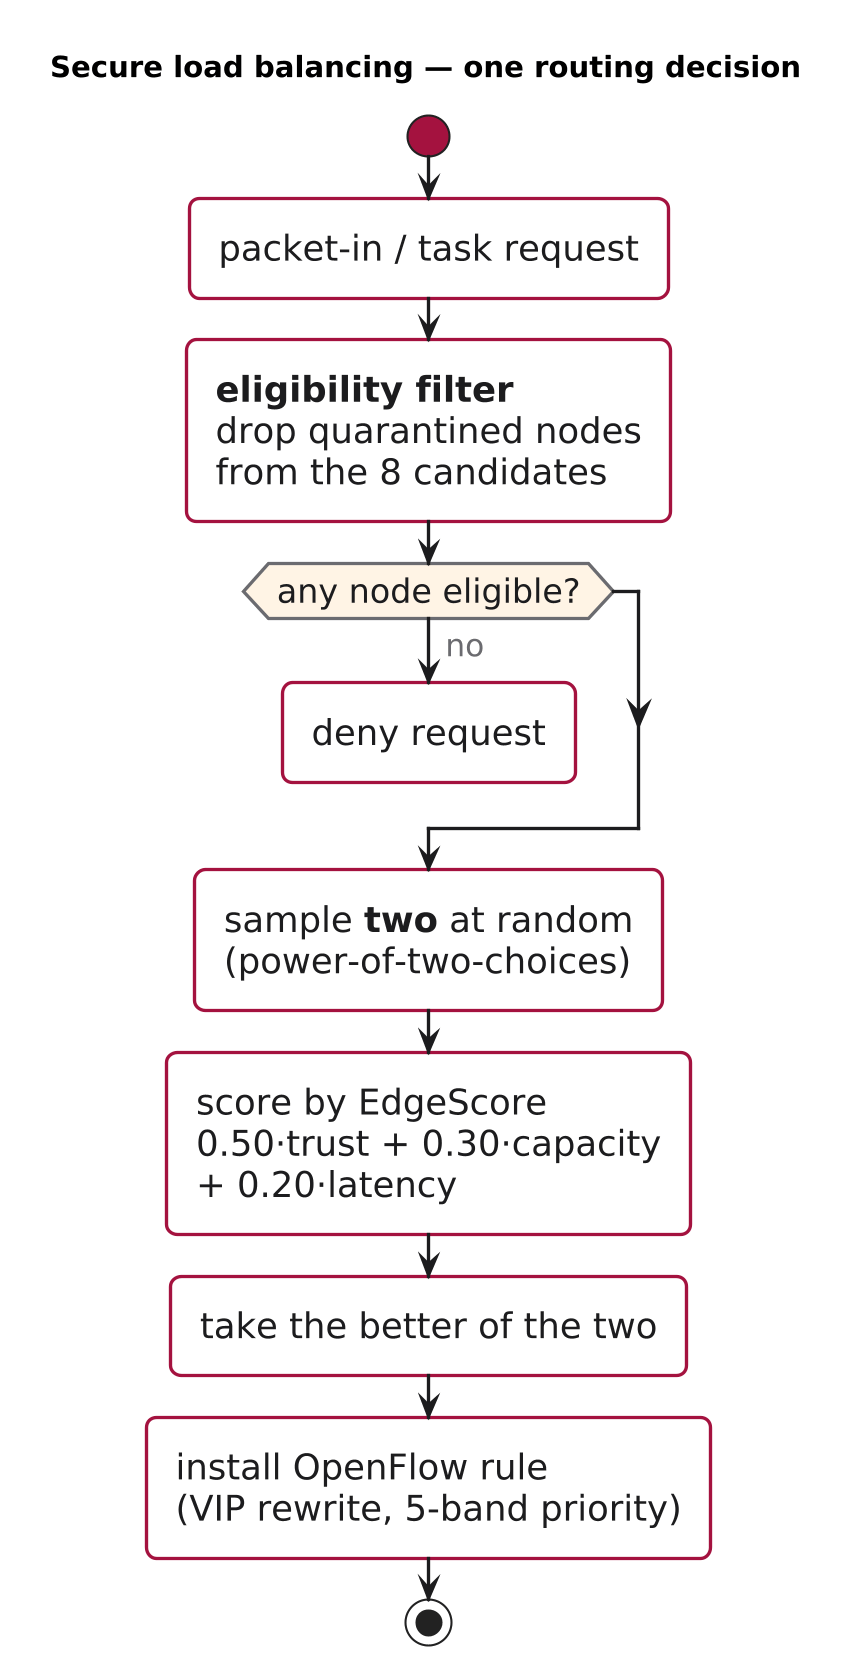
\includegraphics[width=\textwidth,height=0.78\textheight,keepaspectratio]{figures/uml_lb_decision.png}
      \end{column}
      \begin{column}{0.60\textwidth}
        \scriptsize
        \textbf{Why power-of-two-choices, not argmax}\\[2pt]
        Argmax is winner-take-all: every request goes to the single best node
        until its load catches up. We measured it starving the fleet as $N$ grows.
        \vspace{4pt}

        \centering\tiny
        \begin{tabular}{@{}lrr@{}}
          \toprule
          \textbf{At $N=64$ servers} & \textbf{argmax} & \textbf{p2c}\\
          \midrule
          Packet delivery ratio & 10.5\,\% & \textbf{99.7--99.8\,\%}\\
          Tasks lost to timeout & 79\,114  & \textbf{0}\\
          Jain fairness         & 0.75--0.91 & \textbf{$\approx$0.995}\\
          \bottomrule
        \end{tabular}

        \src{data/scalability.csv}

        \vspace{5pt}
        \raggedright\scriptsize
        \textbf{The eligibility filter is the security join.} Quarantined nodes
        are removed from the candidate set \emph{before} scoring, so a trust
        verdict changes routing directly rather than only nudging a weight.

        \vspace{3pt}
        {\tiny\color{gray} Honest caveat: with \emph{no} attacker present we sit
        10.7\,\% behind plain round-robin, because our 1\,s load signal is stale
        relative to $\approx$0.2\,s tasks --- the regime Dahlin [4] describes.}
      \end{column}
    \end{columns}
\end{frame}

\begin{frame}{6. Solution: One Task, End to End}
    \framesubtitle{\rubric{Backend, Frontend, Database \& Core Modules Functional (8 Marks)}}
    \fitfig[0.68]{figures/uml_sequence_task.png}
    \vspace{1pt}
    \centering\tiny
    Enforcement is real: a quarantine verdict becomes an \textbf{OpenFlow drop
    rule}, and in-flight clients are re-dispatched in \textbf{18.13\,ms mean}.
    Every decision is published exactly once to the event bus, so the dashboard
    and all 19 analysis tools read one stream. \src{data/nfr\_report.txt}
\end{frame}

\begin{frame}{6. Solution: Implementation Status}
    \framesubtitle{\rubric{Backend, Frontend, Database \& Core Modules Functional (8 Marks)}}
    \centering\tiny
    \begin{tabular}{@{}p{0.24\textwidth}p{0.56\textwidth}l@{}}
      \toprule
      \textbf{Subsystem / Layer} & \textbf{Current implementation state} & \textbf{Status}\\
      \midrule
      Data plane \& topology   & 1 core + 8 edge OVS switches, 8 edge servers, 40 IoT devices, VIP service model & Functional\\
      SDN control plane        & OpenFlow 1.3: proxy-ARP, per-connection VIP rewrite, 5-band priority table, meters & Functional\\
      Trust engine             & $T=\alpha R+\beta B+\gamma H-\delta A$, EMA $\lambda$=0.85, isolation 0.30, anomaly gate 0.50 & Functional\\
      Secure load balancing    & EdgeScore + power-of-two-choices, eligibility filter, UCB1 online weight tuning & Functional\\
      Security / admission     & PRESENT-80 challenge-response, single-use nonce, source-IP pinning (roster + TOFU) & Functional\\
      Attack detection         & 6 attacks, delayed onset; latency, timeout, honesty and flood tells; windowed classifier & Functional\\
      Blockchain ledger        & SHA-256 chain, Merkle root per block, batch of 10, in-browser re-verification & Functional\\
      Northbound API           & 9 endpoints + SSE stream, standard library only & Functional\\
      Dashboard (frontend)     & Live topology, flow tables, 6 time-series charts, tamper-testable ledger ribbon & Functional\\
      Evaluation \& control arm & 19 analysis tools; complete no-zero-trust control arm; scored comparison & Functional\\
      Test suite               & $\approx$930 test functions across 52 files; CI on every push & Functional\\
      RAFT consensus           & Core + TCP transport + 3-replica live cluster, safety proven. \emph{Not wired into the controller} & \textbf{Partial}\\
      DDoS response            & Detected and classified; throttling not built (needs a per-client-IP OpenFlow path) & \textbf{Partial}\\
      \bottomrule
    \end{tabular}
\end{frame}

% ============================================================ RESULTS
\section{Results}

\begin{frame}{7. Results: The Controlled Comparison}
    \framesubtitle{Baseline 2026-09-05 vs zero-trust 2026-09-08 --- same topology, same 40 devices, same six attacks, same schedule}
    \centering\scriptsize
    \begin{tabular}{@{}lrr@{}}
      \toprule
      \textbf{Metric} & \textbf{Baseline} & \textbf{Zero-trust}\\
      \midrule
      Packet delivery ratio                 & 94.29\,\%      & \textbf{99.43\,\%}\\
      Mean per-device availability (honest) & 85.67\,\%      & \textbf{99.32\,\%}\\
      Honest devices served below 50\,\%    & 5              & \textbf{0}\\
      Tasks lost to timeout                 & 380            & \textbf{32}\\
      p95 task latency                      & 260.0\,ms      & \textbf{147.8\,ms}\\
      Mean task latency                     & \textbf{83.7\,ms} & 92.4\,ms\\
      Throughput                            & 20.74 task/s   & 20.61 task/s\\
      Jain fairness, honest servers only    & 0.689          & \textbf{0.998}\\
      Requests routed to attacker nodes     & 30.5\,\%       & \textbf{13.2\,\%}\\
      Anomalies raised / acted on           & 502 / \textbf{0} & 291 / \textbf{39}\\
      Identity spoof (iot38 $\to$ iot1)     & \textbf{SUCCEEDED} at 19.6\,s & \textbf{REFUSED}\\
      Wrong-key devices admitted            & 2              & \textbf{0}\\
      Trust blocks committed                & --- (no ledger)& 643\\
      \midrule
      \multicolumn{3}{@{}l@{}}{\textbf{Containment, onset $\to$ isolation:} sybil \textbf{7.3\,s} $\cdot$ on-off \textbf{8.3\,s} $\cdot$ blackhole \textbf{9.7\,s} $\cdot$ grayhole \textbf{45.5\,s}}\\
      \multicolumn{3}{@{}l@{}}{\emph{The baseline never contains any of them, because it has no isolation path.}}\\
      \bottomrule
    \end{tabular}

    \vspace{3pt}\tiny
    Mean latency is 8.7\,ms \emph{worse} in our arm --- a small cost in the mean
    to remove the long tail: p95 nearly halves and timeouts fall 92\,\%.
    The grayhole is slowest to contain because a 50\,\% dropper must clear the
    timeout-rate threshold rather than fail outright. \src{data/comparison/comparison.txt, 2026-09-08}
\end{frame}

\begin{frame}{7. Results: Load Distribution and Fairness}
    \framesubtitle{\rubric{Backend, Frontend, Database \& Core Modules Functional (8 Marks)}}
    \fitfig[0.44]{base_model/load/load_share.png}
    \vspace{1pt}
    \fitfig[0.32]{base_model/load/fairness_over_time.png}
    \vspace{1pt}
    \centering\tiny
    Jain over the \emph{whole roster} barely moves (0.622 $\to$ 0.633) and hides
    the result; over the \textbf{four honest servers} it separates hard:
    \textbf{0.689 $\to$ 0.998}. Starving an attacker is correct behaviour, so it
    must not be scored as unfairness. \src{base\_model/plot\_load.py}
\end{frame}

\begin{frame}{7. Results: Per-Server Trust, Both Arms}
    \framesubtitle{\rubric{Backend, Frontend, Database \& Core Modules Functional (8 Marks)}}
    \fitfig[0.56]{base_model/trust/all_servers_trust.png}
    \vspace{2pt}
    \centering\tiny
    Read per node, never as a fleet mean --- averaging a blackhole's collapse
    against seven healthy servers produces a gentle dip and hides the finding.
    Note \textbf{srv3 (sybil) stays high in our arm} at $T=0.699$: the score
    never condemns it, and the anomaly gate is what isolates it. That is Finding 1
    visible in the data. \src{base\_model/trust/}
\end{frame}

\begin{frame}{7. Results: Detection Quality and NFR Validation}
    \framesubtitle{\rubric{Software Architecture, Implementation, Integration \& Tech Stack (5 Marks)}}
    \begin{columns}[T]
      \begin{column}{0.46\textwidth}
        \centering\tiny
        \textbf{Attack detection, 48 subjects}\\[3pt]
        \begin{tabular}{@{}lr@{}}
          \toprule
          \textbf{Measure} & \textbf{Result}\\
          \midrule
          Overall accuracy            & \textbf{47/48 = 97.9\,\%}\\
          Attacks detected at all     & \textbf{8/8}\\
          Placed in the right family  & \textbf{8/8}\\
          Exact label correct         & 7/8\\
          Honest subjects mislabelled & \textbf{0/40}\\
          \bottomrule
        \end{tabular}

        \vspace{3pt}
        \raggedright\tiny
        The one miss: srv6's blackhole was labelled \emph{grayhole} --- the right
        family, one step too mild. Across five catalogued runs exact-label
        accuracy varies 5/8--8/8, so we do not quote a single best run.
        \src{evaluation/attack\_report.py}
      \end{column}
      \begin{column}{0.54\textwidth}
        \centering\tiny
        \textbf{Non-functional requirements --- all four PASS}\\[3pt]
        \begin{tabular}{@{}lllc@{}}
          \toprule
          \textbf{NFR} & \textbf{Target} & \textbf{Measured} & \\
          \midrule
          Routing decision   & $<$200\,ms   & 0.61\,ms mean, p95 0.83 & \textbf{PASS}\\
          Isolation re-dispatch & $<$3\,s   & 18.13\,ms mean, max 29.94 & \textbf{PASS}\\
          Blockchain overhead & $<$15\,\%   & \textbf{0.052\,\%}, 643 blocks & \textbf{PASS}\\
          RAFT commit        & $<$500\,ms   & 4.3--4.8\,ms mean & \textbf{PASS}\\
          \bottomrule
        \end{tabular}

        \vspace{4pt}
        \raggedright\tiny
        \textbf{Two caveats we state ourselves.} The isolation figure is the
        \emph{re-dispatch} time; \emph{detection} is bounded by a 1\,s poll with
        3-poll persistence, so ``$<$3\,s'' is met inclusively at best. And the
        RAFT row is measured on a \textbf{standalone 3-replica cluster, not on
        the controller}. \src{data/nfr\_report.txt}
      \end{column}
    \end{columns}
\end{frame}

\begin{frame}{7. Results: Recorded RAFT Failover}
    \framesubtitle{3 replicas, real TCP, real SIGTERM --- standalone cluster, not the live controller}
    \begin{columns}[T]
      \begin{column}{0.52\textwidth}
        \centering
        \includegraphics[width=\textwidth,height=0.72\textheight,keepaspectratio]{data/figures/raft_failover.png}
      \end{column}
      \begin{column}{0.48\textwidth}
        \scriptsize
        \textbf{What the recording shows}
        \begin{itemize}\itemsep2pt
          \item 853 commits attempted, \textbf{850 succeeded} (99.6\,\%)
          \item Latency mean \textbf{2.6\,ms}, median 2.4, max 19.4
          \item Leader \texttt{n2} killed by SIGTERM at $t=15.0$\,s
          \item \texttt{n1} elected after \textbf{0.21\,s}; service gap 0.21\,s
          \item 3 attempts refused while unreachable --- and refusing is correct
          \item Degraded phase (2 of 3 up) costs only 2.23 $\to$ 3.08\,ms
        \end{itemize}
        \vspace{4pt}
        {\tiny\color{gray} On restart \texttt{n2} rejoins with an \emph{empty}
        log: this is crash-fault tolerance with an in-memory log, not Byzantine
        fault tolerance and not durable storage. We state that before being
        asked.} \src{data/raft\_timeline.jsonl}
      \end{column}
    \end{columns}
\end{frame}

% ============================================================ LIMITATIONS
\section{Limitations \& Future Work}

\begin{frame}{8. Limitations and What Comes Next}
    \scriptsize
    \begin{columns}[T]
      \begin{column}{0.5\textwidth}
        \textbf{Known limitations, stated plainly}
        \begin{itemize}\itemsep3pt
          \item \textbf{RAFT is built, tested and demonstrated --- but not wired
                into the controller.} All 643 blocks of the live run carry
                \texttt{raft\_term = 0}.
          \item \textbf{DDoS is detection-only.} Throttling needs a
                per-client-IP OpenFlow path; we deferred it rather than shipping
                half of it.
          \item \textbf{One live run per configuration}, so no confidence
                intervals on the live figures.
          \item Detection latency is an \textbf{upper bound}, measured from
                controller start.
          \item Scale past 8 servers is a \textbf{queueing simulation}, not a
                live network; all runs are localhost, not multi-host.
        \end{itemize}
      \end{column}
      \begin{column}{0.5\textwidth}
        \textbf{Next steps, in order}
        \begin{enumerate}\itemsep3pt
          \item \textbf{Wire RAFT into the commit path.} Three blockers remain:
                nobody drives the tick; \texttt{commit()} would block an
                OpenFlow handler thread for up to 2\,s; a \texttt{None} return
                is currently discarded silently.
          \item \textbf{Build the per-client-IP throttle} so the flood detector
                has an enforcement path, closing the DDoS story.
          \item \textbf{Repeat the live runs with multiple seeds} to put
                intervals on the headline table.
          \item \textbf{Improve grayhole containment} --- 45.5\,s is our weakest
                result, and a fractional dropper needs a sharper tell than
                timeout rate alone.
        \end{enumerate}
      \end{column}
    \end{columns}
\end{frame}

% ============================================================ TECHNICAL ENRICHMENT
\section{Technical Enrichment}

\begin{frame}{9. Technical Enrichment Activity Choices}
    \framesubtitle{Professional Online Certification Details (Individual Mandatory: 10--20 Hours)}
    \vspace{-2pt}
    \begin{table}
        \centering
        \scriptsize
        \renewcommand{\arraystretch}{1.15}
        \begin{tabular}{|c|p{2.6cm}|p{5.4cm}|p{1.7cm}|c|}
            \hline
            \textbf{S.No} & \textbf{Student Name} & \textbf{Chosen MOOC / Course Title} & \textbf{Platform} & \textbf{Hours} \\
            \hline
            1 & K R Jeevan Raj     & \FIXME{[Course title]} & \FIXME{[Platform]} & \FIXME{[--]} \\
            \hline
            2 & Aravind Kumar M    & Software Defined Networking \newline {\tiny\color{gray}The University of Chicago} & Coursera & \FIXME{30 Hrs} \\
            \hline
            3 & Arjun Krishnakumar & Cisco ACI Training: Design and Implement Data Center SDN & Udemy & \FIXME{[--]} \\
            \hline
            4 & Ashwin Kumar RM    & Network Security \newline {\tiny\color{gray}Cisco Learning and Certifications} & Coursera & 12 Hrs \\
            \hline
            5 & Bhuvanesh S        & \FIXME{[Course title]} & \FIXME{[Platform]} & \FIXME{[--]} \\
            \hline
        \end{tabular}
    \end{table}
    \vspace{4pt}
    \scriptsize
    \textbf{Requirement:} each student completes one approved 10--20 hour online
    certification from a recognised platform, relevant to the project.\\[3pt]
    {\color{gray} The three chosen so far map directly onto the parts of the
    system their holders own: \emph{Software Defined Networking} underpins the
    OpenFlow control plane, \emph{Cisco ACI} covers data-centre SDN and policy
    fabric, and \emph{Network Security} covers the zero-trust admission and
    detection path.}
\end{frame}

% ============================================================ REFERENCES
%  Numbering [1]-[13] is IDENTICAL to Appendix B of the project report, so a
%  citation means the same thing in the deck, the report and the paper.
%  [14]-[21] are additions used by the deck. Plain \item[...] labels are used
%  rather than \bibliography{ref}: there is no ref.bib in this repository,
%  IEEEtran.bst is not installed, and the "why we cite it" annotations below
%  would not survive a .bst anyway.
% ============================================================
\section{References}

\begin{frame}[allowframebreaks]{References I: Zero Trust and Load Balancing}
    \framesubtitle{Numbering matches Appendix B of the project report}
    \scriptsize

    \textbf{Zero Trust and trust-aware edge computing}
    \begin{itemize}\itemsep1.5pt
        \item[{[1]}] S. Rose, O. Borchert, S. Mitchell and S. Connelly, ``Zero Trust Architecture,'' \emph{NIST Special Publication 800-207}, National Institute of Standards and Technology, Aug. 2020.\\
          {\color{gray}$\rightarrow$ The doctrine we implement, and the gap we claim. It mandates continuous verification but specifies no mechanism for verifying the \emph{serving infrastructure}.}
        \item[{[11]}] B. Ali, M. A. Gregory and S. Li, ``Trust-aware task load balancing in multi-access edge computing based on blockchain and a zero trust security capability framework,'' \emph{Trans. Emerging Telecommunications Technologies}, vol.~34, no.~12, e4845, 2023. DOI 10.1002/ett.4845.\\
          {\color{gray}$\rightarrow$ The closest prior work, with the same three ingredients of zero trust, blockchain and MEC load balancing. We differ in enforcing the verdict in the data plane and in measuring against a control arm.}
        \item[{[12]}] ``Securing edge based smart city networks with software defined networking and zero trust architecture (TREN),'' \emph{J. Network and Computer Applications}, 2025. DOI 10.1016/j.jnca.2025.104318.\\
          {\color{gray}$\rightarrow$ The smart-city and SDN application domain.}
        \item[{[13]}] M. Huang, Z. Li, F. Xiao, S. Long and A. Liu, ``Trust Mechanism-Based Multi-Tier Computing System for Service-Oriented Edge-Cloud Networks,'' \emph{IEEE Trans. Dependable and Secure Computing}, vol.~21, no.~4, pp.~1639-1651, 2024. DOI 10.1109/TDSC.2023.3285927.\\
          {\color{gray}$\rightarrow$ Trust scoring for edge task placement. This is the score-only design whose arithmetic ceiling our Finding 1 characterises.}
        \item[{[19]}] ETSI GS MEC 003, ``Multi-access Edge Computing (MEC); Framework and Reference Architecture,'' V3.1.1, 2022.\\
          {\color{gray}$\rightarrow$ The deployment mapping: controller to MEC orchestrator, edge servers to MEC hosts, IoT clients to UE.}
    \end{itemize}

    \vspace{3pt}
    \textbf{Load balancing: why we replaced argmax with power-of-two-choices}
    \begin{itemize}\itemsep1.5pt
        \item[{[2]}] M. Mitzenmacher, ``The Power of Two Choices in Randomized Load Balancing,'' \emph{IEEE Trans. Parallel and Distributed Systems}, vol.~12, no.~10, pp.~1094-1104, 2001. DOI 10.1109/71.963420.\\
          {\color{gray}$\rightarrow$ The source of our fix. Sampling two candidates and taking the better one gives far better tail behaviour than picking the single best.}
        \item[{[14]}] Y. Azar, A. Z. Broder, A. R. Karlin and E. Upfal, ``Balanced Allocations,'' \emph{SIAM J. Computing}, vol.~29, no.~1, pp.~180-200, 1999.\\
          {\color{gray}$\rightarrow$ The originating balanced-allocations result behind [2].}
        \item[{[3]}] M. Mitzenmacher, ``How Useful Is Old Information?,'' \emph{IEEE Trans. Parallel and Distributed Systems}, vol.~11, no.~1, pp.~6-20, 2000. DOI 10.1109/71.824633.\\
          {\color{gray}$\rightarrow$ Herd behaviour caused by stale load information. Our poll interval is 1\,s while tasks finish in about 0.2\,s, which is the regime this paper describes.}
        \item[{[4]}] M. Dahlin, ``Interpreting Stale Load Information,'' \emph{IEEE Trans. Parallel and Distributed Systems}, vol.~11, no.~10, pp.~1033-1047, 2000. DOI 10.1109/71.888643.\\
          {\color{gray}$\rightarrow$ \textbf{This explains the one place we lose.} Stale least-loaded performs worse than random, which is why we sit 10.7\,\% behind round-robin in the no-attack case.}
        \item[{[9]}] R. Jain, D.-M. Chiu and W. Hawe, ``A Quantitative Measure of Fairness and Discrimination for Resource Allocation in Shared Computer Systems,'' \emph{DEC Research Report TR-301}, 1984.\\
          {\color{gray}$\rightarrow$ The fairness index reported in Section 7 (0.689 to 0.998, honest servers only).}
        \item[{[20]}] J. D. C. Little, ``A Proof for the Queuing Formula $L = \lambda W$,'' \emph{Operations Research}, vol.~9, no.~3, pp.~383-387, 1961.\\
          {\color{gray}$\rightarrow$ The diagnostic that proved a live run's occupancy was fabricated rather than real.}
    \end{itemize}
\end{frame}

\begin{frame}[allowframebreaks]{References II: Security, Consensus and Method}
    \framesubtitle{Numbering matches Appendix B of the project report}
    \scriptsize

    \textbf{Lightweight cryptography and the tamper-evident ledger}
    \begin{itemize}\itemsep1.5pt
        \item[{[5]}] A. Bogdanov, L. R. Knudsen, G. Leander, C. Paar, A. Poschmann, M. J. B. Robshaw, Y. Seurin and C. Vikkelsoe, ``PRESENT: An Ultra-Lightweight Block Cipher,'' in \emph{Cryptographic Hardware and Embedded Systems (CHES 2007)}, LNCS 4727, pp.~450-466, 2007.\\
          {\color{gray}$\rightarrow$ The cipher behind device admission, and the published test vectors our implementation is checked against.}
        \item[{[18]}] ISO/IEC 29192-2:2019, \emph{Information security, lightweight cryptography, Part~2: Block ciphers}.\\
          {\color{gray}$\rightarrow$ The standardisation that makes PRESENT-80 a defensible choice for constrained devices, and the framing for its 80-bit key being below modern margins.}
        \item[{[6]}] R. C. Merkle, ``A Digital Signature Based on a Conventional Encryption Function,'' in \emph{Advances in Cryptology (CRYPTO '87)}, LNCS 293, pp.~369-378, 1988.\\
          {\color{gray}$\rightarrow$ The Merkle tree giving per-record proofs. Our \texttt{\_hash\_pair} was fixed to positional concatenation so that proofs are order-sensitive, as the construction requires.}
        \item[{[7]}] D. Ongaro and J. Ousterhout, ``In Search of an Understandable Consensus Algorithm,'' in \emph{Proc. USENIX Annual Technical Conf.}, pp.~305-319, 2014.\\
          {\color{gray}$\rightarrow$ RAFT. Safety properties R-01 to R-18 are tested against this paper's statements. It is crash-fault tolerant and \emph{not} Byzantine, a distinction we state before being asked.}
    \end{itemize}

    \vspace{3pt}
    \textbf{SDN platform}
    \begin{itemize}\itemsep1.5pt
        \item[{[8]}] N. McKeown, T. Anderson, H. Balakrishnan, G. Parulkar, L. Peterson, J. Rexford, S. Shenker and J. Turner, ``OpenFlow: Enabling Innovation in Campus Networks,'' \emph{ACM SIGCOMM Computer Communication Review}, vol.~38, no.~2, pp.~69-74, 2008.\\
          {\color{gray}$\rightarrow$ The protocol our decisions are installed as, and the source of Finding 3: once a rule is installed, matching packets never return to the controller.}
        \item[{[10]}] B. Lantz, B. Heller and N. McKeown, ``A Network in a Laptop: Rapid Prototyping for Software-Defined Networks,'' in \emph{Proc. 9th ACM SIGCOMM Workshop on Hot Topics in Networks (HotNets)}, 2010.\\
          {\color{gray}$\rightarrow$ Mininet, the emulation testbed. It is why we say ``demonstrated in an emulated network'' and never ``proven in production''.}
    \end{itemize}

    \vspace{3pt}
    \textbf{Learning and statistical method}
    \begin{itemize}\itemsep1.5pt
        \item[{[15]}] P. Auer, N. Cesa-Bianchi and P. Fischer, ``Finite-time Analysis of the Multiarmed Bandit Problem,'' \emph{Machine Learning}, vol.~47, no.~2/3, pp.~235-256, 2002.\\
          {\color{gray}$\rightarrow$ UCB1, the online EdgeScore weight optimiser. A classical bandit and \emph{not} deep reinforcement learning, because weight tuning is an exploration problem when no labelled data exists at runtime.}
        \item[{[16]}] F. Wilcoxon, ``Individual Comparisons by Ranking Methods,'' \emph{Biometrics Bulletin}, vol.~1, no.~6, pp.~80-83, 1945.\\
          {\color{gray}$\rightarrow$ The paired signed-rank test behind every $p$-value we report. Chosen over a paired $t$-test because our outcomes are bounded rates, skewed and zero-inflated.}
        \item[{[17]}] S. Holm, ``A Simple Sequentially Rejective Multiple Test Procedure,'' \emph{Scandinavian J. Statistics}, vol.~6, no.~2, pp.~65-70, 1979.\\
          {\color{gray}$\rightarrow$ The multiple-comparison correction. One system against four baselines is four tests, so the family-wise false-positive rate is about 19\,\% rather than 5\,\%. Holm is uniformly more powerful than Bonferroni for the same guarantee.}
        \item[{[21]}] M. T. Nygard, \emph{Release It!: Design and Deploy Production-Ready Software}, 2nd ed., Pragmatic Bookshelf, 2018.\\
          {\color{gray}$\rightarrow$ The circuit-breaker pattern. Our \emph{probation} mechanism is its half-open leg, and it is what stopped quarantine being an absorbing state.}
    \end{itemize}
\end{frame}

% ============================================================ THANK YOU
\begin{frame}
    \centering
    {\Huge \textbf{\textcolor{amritaMaroon}{Thank You}}}\\[10pt]
    {\footnotesize Questions welcome --- including the ones about what we have not finished.}
\end{frame}

% ============================================================ BACKUP
\section*{Backup}

\begin{frame}{Backup: Design Patterns and Engineering Decisions}
    \framesubtitle{\rubric{Software Architecture, Implementation, Integration \& Tech Stack (5 Marks)}}
    \centering\tiny
    \begin{tabular}{@{}p{0.18\textwidth}p{0.24\textwidth}p{0.50\textwidth}@{}}
      \toprule
      \textbf{Pattern} & \textbf{Where} & \textbf{Justification}\\
      \midrule
      Layered architecture & L1 to L5 & The trust engine must be callable with enforcement removed --- that is what makes the control arm a controlled experiment rather than a second codebase\\
      Strategy & \texttt{edge\_selector}, \texttt{static\_router} & Routing policy is a config key (\texttt{selection: p2c}), so the two arms differ by a key, not a fork\\
      Protocol / structural typing & \texttt{CommitBackend}, \texttt{Transport} & \texttt{RaftBackend} is a drop-in for \texttt{LocalLedgerBackend}; \texttt{RaftNode} did not change at all to gain a TCP transport\\
      Observer / pub-sub & \texttt{EventBus} $\to$ SSE + JSONL & Every decision is published exactly once; dashboard and analysis tools read one stream\\
      Pure function & \texttt{attack\_classifier} & No I/O, no locks, no state, so live and offline verdicts come from one implementation\\
      Decorator & \texttt{TimingCommitBackend} & Commit cost is measured without the ledger knowing it is being timed\\
      Multi-armed bandit (UCB1) & \texttt{ai\_optimizer} & Weight tuning is an exploration problem rather than a training problem, because no labelled data exists at runtime\\
      \bottomrule
    \end{tabular}

    \vspace{3pt}\tiny
    \textbf{Stack:} Python 3.14 $\cdot$ os-ken (Ryu fork) $\cdot$ Mininet + Open vSwitch, OpenFlow 1.3 $\cdot$
    stdlib \texttt{ThreadingHTTPServer} + SSE $\cdot$ PRESENT-80 $\cdot$ SHA-256/Merkle $\cdot$ pytest.
\end{frame}

\begin{frame}{Backup: Data Integrity, Concurrency and Error Handling}
    \centering\tiny
    \begin{tabular}{@{}p{0.24\textwidth}p{0.70\textwidth}@{}}
      \toprule
      \textbf{Concern} & \textbf{Mechanism}\\
      \midrule
      Ledger integrity & SHA-256 chain + Merkle root per block; the browser recomputes the hash itself rather than trusting the controller's \texttt{valid} flag\\
      Deterministic replication & Log entries carry only content; \texttt{index}, \texttt{previous\_hash} and \texttt{merkle\_root} are recomputed per replica at apply time --- the fix for a non-deterministic genesis block and a stale ledger snapshot taken at proposal time\\
      Concurrency & One \texttt{RLock} guards \texttt{RaftNode}/\texttt{Ledger} (re-entrant, because \texttt{apply\_fn} re-enters it); a second lock serialises whole \texttt{commit()} calls; \texttt{commit()} releases the first while waiting, or the driver thread deadlocks\\
      Trust-state consistency & All mutation under one lock; the invariant \texttt{sum(\_inflight) == len(\_dispatches)} is asserted, after a register leak once fabricated load on honest nodes\\
      Replay resistance & Nonces are single-use (popped on first verification) and expire after 30\,s\\
      Identity integrity & The fleet key is shared, so PRESENT-80 authenticates possession of the key rather than the device. That gap is closed by source-IP pinning against a provisioned roster, with TOFU as the fallback\\
      Error handling & Structured \texttt{AuthError(kind)}; a 403 also \emph{publishes} an event, so a refusal is visible in the recording; meters degrade to allow/quarantine where unsupported, logged once\\
      \bottomrule
    \end{tabular}
\end{frame}

\begin{frame}{Backup: The Statistical Study and Its Negative Results}
    \scriptsize
    \textbf{600 paired seeded runs} --- 5 strategies $\times$ 4 scenarios $\times$ 30 seeds.
    {\color{gray}This is a \textbf{simulation harness driving the real selector and
    calculator}, not a Mininet run --- a different instrument from the live
    comparison in Section 7.}
    \begin{itemize}\itemsep2pt
      \item 14 of 16 comparisons favour the system, $p_{\mathrm{adj}} = 7.45\times10^{-9}$, rank-biserial $r = +1.00$
      \item SLO-violation reduction vs the trust-ablated variant: sybil $-15.1$\,\%, drop $-25.3$\,\%, both $-29.8$\,\%
      \item Failure-rate reduction $-97.7$\,\%; malicious-traffic share $-97.5$ to $-97.7$\,\%
    \end{itemize}
    \vspace{3pt}
    \textbf{The results that did not go our way, reported because they are ours}
    \begin{itemize}\itemsep2pt
      \item \textbf{We lose twice, both with no attacker present:} $-10.7$\,\% vs round-robin and $-4.8$\,\% vs random. Cause isolated by a poll-interval sweep: 1\,s load-signal staleness, exactly the effect Dahlin [4] describes. It disappears at a 0.01\,s poll.
      \item \textbf{A capacity cliff at $N=4$ servers with 2 attackers} --- with half the fleet hostile the system loses the SLO metric. It is fine from $N=6$.
      \item \textbf{The Random-Forest warm start did not beat static weights} (2 of 4 scenarios significant, and \emph{against} it). We report UCB1's online tuning as the working mechanism and the RF path as a measured dead end.
      \item \textbf{Isolation is 3.0\,s median, 4.0\,s max in the harness} --- the ``$<$3\,s'' target is met inclusively at best, by construction of the 1\,s poll.
    \end{itemize}
\end{frame}

\end{document}
